\newif\ifglobal

%%%%%%%%%%%%%%%%%%%%%%%
%%% Compile to view %%%
%%%%%%%%%%%%%%%%%%%%%%%

%%%%%%%%%%%%%%%%%%%%%%%%%%%%%%%%%%%%%%%%%%%%%%%%%%%
%%% Readme:                                     %%%
%%% https://www.overleaf.com/read/bwdjvfjksvjy/ %%%
%%%%%%%%%%%%%%%%%%%%%%%%%%%%%%%%%%%%%%%%%%%%%%%%%%%

% >>> M?: marks a module setting number or important notice

% >>> M4: Set {./relative-path} to external files for this module <<<
\def \modulefiles {./03-SYSMEM}
% To add an external file, use:
% (Replace '---' with actual filename)
% '\input{\modulefiles/tables/---.tex}' for tables
% '\includegraphics{\modulefiles/figures/---}' for figures
% '\subfile{\modulefiles/---}' for register files


% >>> M1: This module is in global project? <<<
% 'YES' - uncomment; 'NO' - comment out
\globaltrue

\ifglobal
    \documentclass[main\_\_EN.tex]{subfiles}

\else
    \documentclass[openany, 10pt]{book}

    % >>> M2: In ./00-shared/preamble-trm-module, also find
    %         settings for visibility of todo notes, watermark <<<
    \usepackage{preamble-trm-module}

    % >>> M3: Temporary labels in English,
    %         you can add your own labels there <<<
    \myexternaldocument{./00-shared/temp-labels-en}

\fi %\ifglobal


\setcounter{secnumdepth}{4}


% >>> M5: If this module needs any updates in
% './00-shared/preamble-trm-module.sty'
% (include additional package, etc.), contact your module PM
% or create the file './00-shared/changelog.tex' make the
% necessary updates yourself and document them in this file <<<


\begin{document}


% Sets language into which pre-defined bits of text are translated
\selectlanguage{english}

% Do not delete this block
\ifglobal
% Add the following front matter if
% this module is outside of global project
\else
    \InputIfFileExists{readme}{}{}
    {\let\clearpage\relax \listoftodos}
    {\let\clearpage\relax \listofdonetodos}
    \tableofcontents
    %\listoftables
    %\listoffigures
\fi


%%%%%%%%%%%%%%%%%%%%%%%%%
%%% TRM Module Begins %%%
%%%%%%%%%%%%%%%%%%%%%%%%%

\hypertarget{sysmem}{}
\chapter{System and Memory}
\label{mod:sysmem}


\section{Overview}

The \chipname{} is an ultra-low-power and highly-integrated system with a 32-bit RISC-V single-core processor and a four-stage pipeline that operates at up to 120 MHz. All internal memory, external memory, and peripherals are located on the CPU buses.



\section{Features}

\chipname{}'s system and memory has the following features:

\begin{itemize}
    \item {\bfseries Address Space}
        \begin{itemize}
    	    \item 848 KB of internal memory address space accessed from the instruction bus
            \item 576 KB of internal memory address space accessed from the data bus
    	    \item 828 KB of peripheral address space
    	    \item 4 MB of external memory virtual address space accessed from the instruction bus
    	    \item 4 MB of external memory virtual address space accessed from the data bus
    	    \item 576 KB of internal DMA address space
        \end{itemize}
    \item {\bfseries Internal Memory}
        \begin{itemize}
            \item 576 KB of internal ROM
	        \item 272 KB of internal SRAM
	    \end{itemize}
    \item {\bfseries External Memory}
        \begin{itemize}
            \item Supports up to 16 MB external flash
	    \end{itemize}
    \item {\bfseries Peripheral Space}
        \begin{itemize}
           \item 22 modules/peripherals in total
        \end{itemize}
    \item {\bfseries GDMA}
        \begin{itemize}
            \item 2 GDMA-supported modules/peripherals
        \end{itemize}
\end{itemize}

Figure \ref{fig:sysmem-address-mapping-structure} illustrates the system structure and address mapping.

\begin{figure}[H]
    \centering
    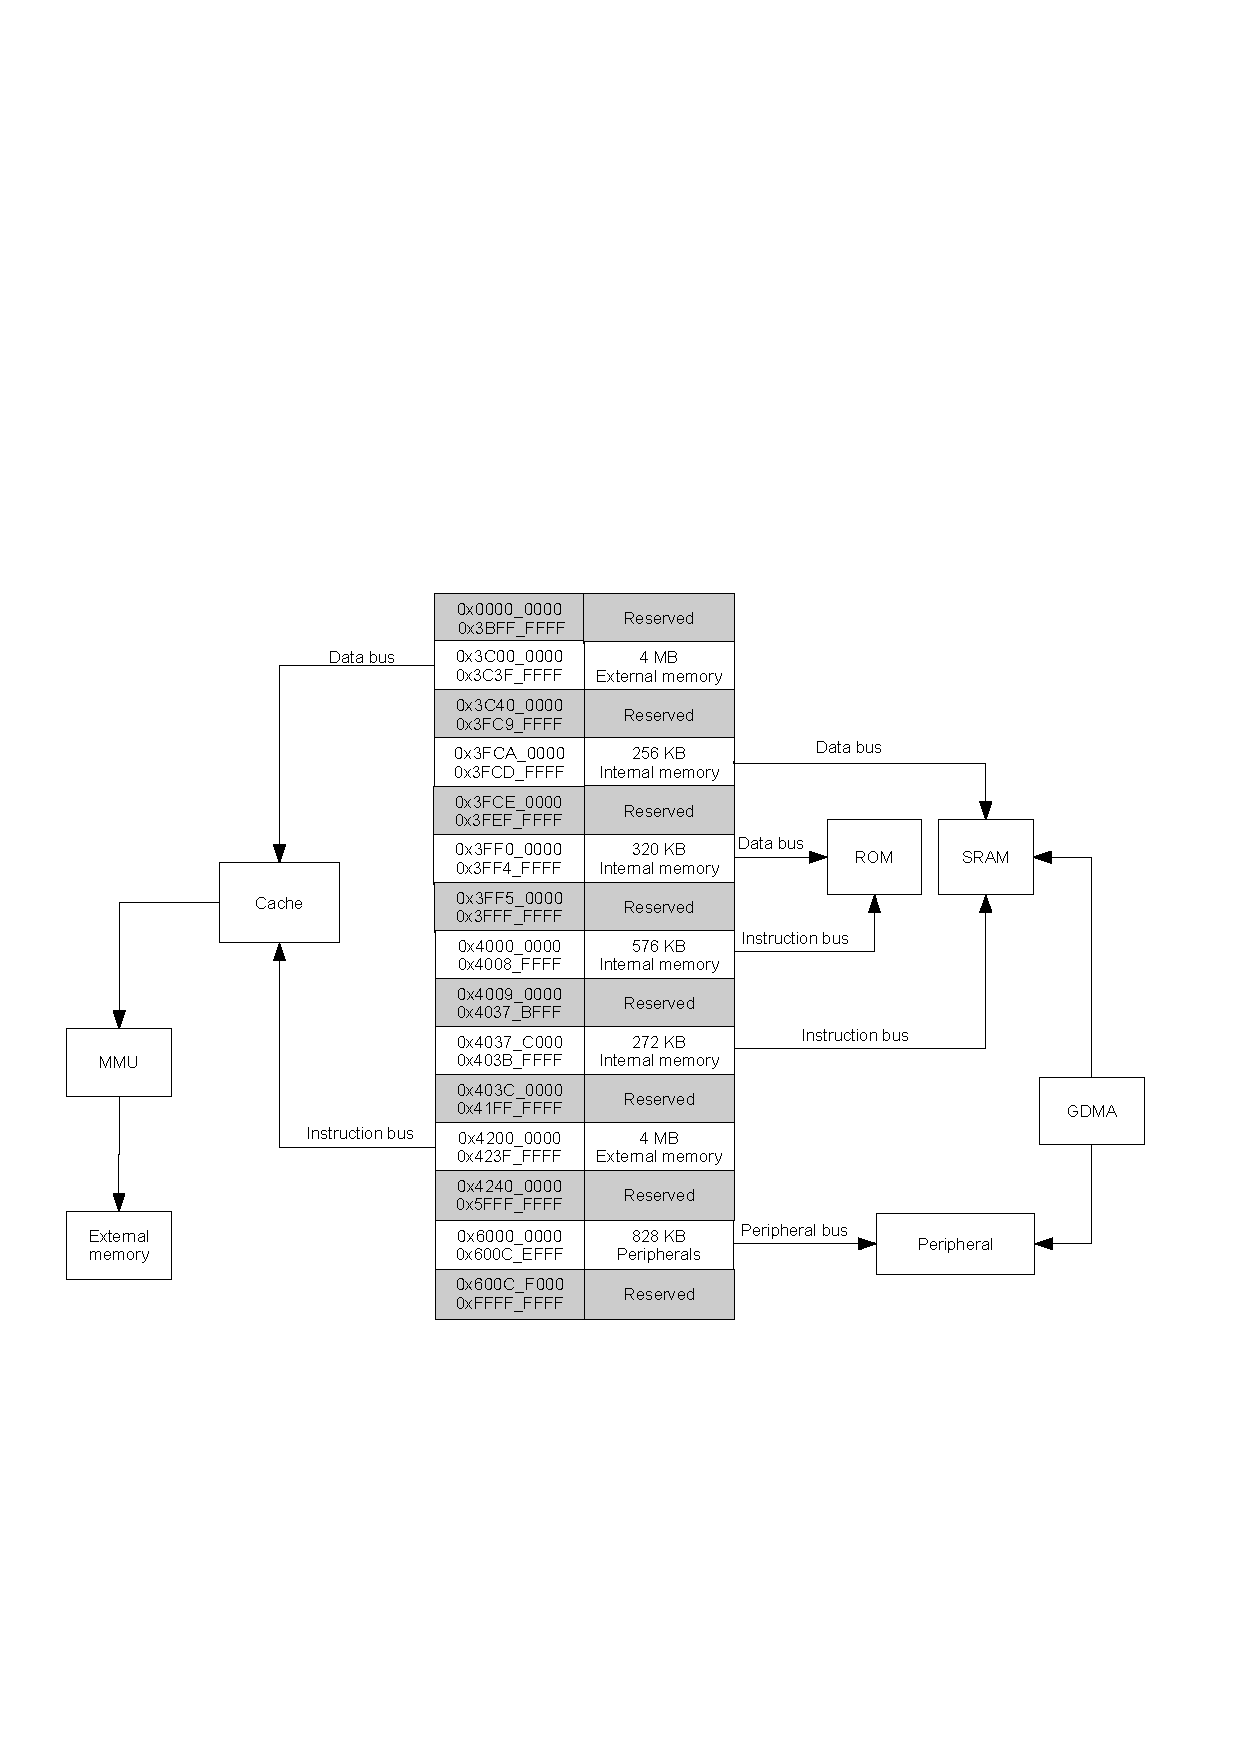
\includegraphics[width=1.0\textwidth]{./03-SYSMEM/figures/03-SYSMEM-addr-mapping.pdf}
    \caption{System Structure and Address Mapping}
    \label{fig:sysmem-address-mapping-structure}
\end{figure}

\begin{tiplisting}
\vspace{-2em}
\begin{itemize}
    \item The address space with gray background is not available to users.
    \item The range of addresses available in the address space may be larger than the actual available memory of a particular type.
\end{itemize}

\end{tiplisting}

\section{Functional Description}

\subsection{Address Mapping}

Addresses below 0x4000\_0000 are accessed using the data bus. Addresses in the range of 0x4000\_0000 \verb+~+ 0x4FFF\_FFFF are accessed using the instruction bus. Addresses over and including 0x5000\_0000 are accessed using the peripheral bus.

Both the data bus and instruction bus are little-endian. The CPU can access data via the data bus using single-byte, double-byte, four-byte alignment. The CPU can also access data via the instruction bus, but only in four-byte aligned manner.


The CPU can:
\begin{itemize}
\item directly access the internal memory via both the data bus and instruction bus;
\item  access the external memory which is mapped into the virtual address space via cache;
\item directly access modules/peripherals via the peripheral bus.
\end{itemize}

Figure \ref{fig:sysmem-address-mapping-structure} shows the address ranges on the data bus, instruction bus and peripheral bus as well as their corresponding target memory.

Some internal and external memory can be accessed via both the data bus and instruction bus. In such cases, the CPU can access the same memory using multiple addresses.


\subsection{Internal Memory}
\label{para:sysmem-internal-memory}

The \chipname{} consists of the following two types of internal memory:

\begin{itemize}
    \item Internal ROM (576 KB): The Internal ROM of the \chipname{} is a read-only memory which cannot be programmed. Internal ROM contains the ROM code (software instructions and some software read-only data) of some low-level system software.
    \item Internal SRAM (272 KB): The Internal Static RAM (SRAM) is a volatile memory that can be quickly accessed by the CPU (generally within a single CPU clock cycle).
    \begin{itemize}
        \item A part of the SRAM can be configured to operate as a cache for external memory access.
        \item Some parts of the SRAM can only be accessed via the CPU's instruction bus.
        \item Some parts of the SRAM can be accessed via both the CPU's instruction bus and the CPU's data bus.
    \end{itemize}
\end{itemize}

Based on the two different types of internal memory described above, the internal memory of the \chipname{} is split into two segments: Internal ROM (576 KB) and Internal SRAM (272 KB).


However, within each segment, there may be different bus access restrictions (e.g., some parts of the segment may only be accessible by the CPU's data bus). Therefore, segments are also further divided into parts. Table \ref{tab:sysmem-internal-memory} describes each part of internal memory and their address ranges on the data bus and instruction bus.


\begin{longtable}[c]{|p{3.5cm}|c|c|r|c| }
    \caption{Internal Memory Address Mapping}
    \label{tab:sysmem-internal-memory}
       \\\hline
        \rowcolor{lightgray}
        & \multicolumn{2}{c|}{\textbf{Boundary Address}} & & \\\cline{2-3}

        \rowcolor{lightgray}
        \multirow{-2}*{\textbf{Bus Type}} & \textbf{Low Address} & \textbf{High Address} & \multirow{-2}*{\textbf{Size (KB)}} & \multirow{-2}*{\textbf{Target}} \\\hline
        \endfirsthead

        \multicolumn{5}{c}{\bfseries \tablename\ \thetable{} -- cont'd from previous page}\\\hline

        \rowcolor{lightgray}
        & \multicolumn{2}{c|}{\textbf{Boundary Address}} & & \\\cline{2-3}

         \rowcolor{lightgray}
        \multirow{-2}*{\textbf{Bus Type}} & \textbf{Low Address} & \textbf{High Address} & \multirow{-2}*{\textbf{Size (KB)}} & \multirow{-2}*{\textbf{Target}} \\\hline
        \endhead

    \multicolumn{5}{r}{\textbf{Cont'd on next page}} \\
    \endfoot
    \endlastfoot

        \multirow{2}*{Data bus} & 0x3FF0\_0000 & 0x3FF4\_FFFF & 320  & Internal ROM 1  \\\cline{2-5}
                            & 0x3FCA\_0000 & 0x3FCD\_FFFF & 256  & Internal SRAM 1  \\\cline{2-5}
        \hline
        \multirow{4}*{Instruction bus} & 0x4000\_0000 & 0x4003\_FFFF & 256  & Internal ROM 0 \\\cline{2-5}
                            & 0x4004\_0000 & 0x4008\_FFFF & 320  & Internal ROM 1 \\\cline{2-5}
    	                    & 0x4037\_C000 & 0x4037\_FFFF &  16  & Internal SRAM 0 \\\cline{2-5}
    	                    & 0x4038\_0000 & 0x403B\_FFFF & 256  & Internal SRAM 1 \\\hline
\end{longtable}




{\bfseries 1. Internal ROM 0}

Internal ROM 0 is a 256 KB, read-only memory space, addressed by the CPU only through the instruction bus via 0x4000\_0000 \verb+~+ 0x4003\_FFFF, as shown in Table \ref{tab:sysmem-internal-memory}.

{\bfseries 2. Internal ROM 1}
\label{other:sysmem-internal-rom1}

Internal ROM 1 is a 320 KB, read-only memory space, addressed by the CPU through the instruction bus via 0x4004\_0000 \verb+~+ 0x4008\_FFFF or through the data bus via 0x3FF0\_0000 \verb+~+ 0x3FF4\_FFFF in the same order, as shown in Table \ref{tab:sysmem-internal-memory}.

This means, for example, address 04004\_0000 and 0x3FF0\_0000 correspond to the same word, 0x4004\_0004 and 0x3FF0\_0004 correspond to the same word, 0x4004\_0008 and 0x3FF0\_0008 correspond to the same word, etc.



{\bfseries 3. Internal SRAM 0}
\label{other:sysmem-internal-sram-0}

Internal SRAM 0 is a 16 KB, read-and-write memory space, addressed by the CPU through the instruction bus via the range described in Table \ref{tab:sysmem-internal-memory}.

This memory can be configured as instruction cache to store cache instructions or read-only data of the external memory. In this case, the configured memory cannot be accessed by the CPU.


{\bfseries 4. Internal SRAM 1}

Internal SRAM 1 is a 256 KB, read-and-write memory space, addressed by the CPU through the data bus or instruction bus, in the same order (the same meaning as the explanation in \ref{other:sysmem-internal-sram-0} \textit{Internal ROM 1}), via the ranges described in Table \ref{tab:sysmem-internal-memory}.


\subsection{External Memory}
\label{para:sysmem-external-memory}

\chipname{} supports SPI, Dual SPI, Quad SPI, and QPI interfaces that allow connection to multiple external flash chips. The chip supports hardware manual encryption and automatic decryption based on XTS-AES algorithm to protect user programs and data in the external flash.


\subsubsection{External Memory Address Mapping}

The CPU accesses the external memory via the cache. According to the MMU (Memory Management Unit) settings, the cache maps the CPU's address to the external memory's physical address. Due to this address mapping, the \chipname{} can address up to 16 MB external flash.


Using the cache, \chipname{} is able to support the following address space mappings. Note that the instruction bus address space (4 MB) and the data bus address space (4 MB) is always shared.

\begin{itemize}
    \item Up to 4 MB instruction bus address space can be mapped into the external flash. The mapped address space is organized as individual 64-KB blocks.
    \item Up to 4 MB data bus (read-only) address space can be mapped into the external flash. The mapped address space is organized as individual 64-KB blocks.
\end{itemize}

Table \ref{tab:sysmem-external-memory} lists the mapping between the cache and the corresponding address ranges on the data bus and instruction bus.

 \begin{longtable}[c]{|p{3cm}|c|c|r|c| }
  \caption{External Memory Address Mapping}
  \label{tab:sysmem-external-memory}
  \\\hline

    \rowcolor{lightgray}
        & \multicolumn{2}{c|}{\textbf{Boundary Address}} & & \\\cline{2-3}

    \rowcolor{lightgray}
        \multirow{-2}*{\textbf{Bus Type}} & \textbf{Low Address} & \textbf{High Address} & \multirow{-2}*{\textbf{Size (MB)}} & \multirow{-2}*{\textbf{Target}} \\\hline
    \endfirsthead

    \multicolumn{5}{c}{\bfseries \tablename\ \thetable{} -- cont'd from previous page}\\\hline

    \rowcolor{lightgray}
        & \multicolumn{2}{c|}{\textbf{Boundary Address}} & & \\\cline{2-3}

    \rowcolor{lightgray}
        \multirow{-2}*{\textbf{Bus Type}} & \textbf{Low Address} & \textbf{High Address} & \multirow{-2}*{\textbf{Size (MB)}} & \multirow{-2}*{\textbf{Target}} \\\hline
    \endhead

    \multicolumn{5}{r}{\textbf{Cont'd on next page}} \\
    \endfoot
    \endlastfoot


    Data bus (read-only)        & 0x3C00\_0000 & 0x3C3F\_FFFF &  4  & Uniform Cache \\\hline
    Instruction bus                & 0x4200\_0000 & 0x423F\_FFFF &  4  & Uniform Cache \\\hline

\end{longtable}




\subsubsection{Cache}


As shown in Figure \ref{fig:sysmem-cache-arch}, \chipname{} has a read-only uniform cache which is four-way set-associative, its size is 16 KB and its block size is 32 bytes. When cache is active, some internal memory space will be occupied by cache (see Internal SRAM 0 in Section \ref{other:sysmem-internal-sram-0}). 

The uniform cache is accessible by the instruction bus and the data bus at the same time, but can only respond to one of them at a time. When a cache miss occurs, the cache controller will initiate a request to the external memory.



\begin{figure}[H]
    \centering
    \fbox{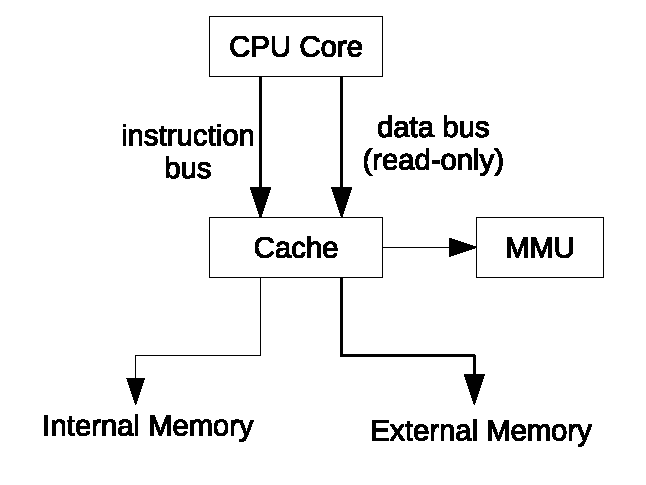
\includegraphics[width=0.5\textwidth]{./03-SYSMEM/figures/03-SYSMEM-cache-arch__EN.eps}}
     \caption{Cache Structure}
    \label{fig:sysmem-cache-arch}
\end{figure}

\subsubsection{Cache Operations}

\chipname{} cache supports the following operation:

\begin{enumerate}
\item \textbf{Invalidate}: This operation is used to clear valid data in the cache. After this operation is completed, the data will only be stored in the external memory. The CPU needs to access the external memory in order to read this data. There are two types of invalidate-operation: automatic invalidation (Auto-Invalidate) and manual invalidation (Manual-Invalidate). Manual-Invalidate is performed only on data in the specified area in the cache, while Auto-Invalidate is performed on all data in the cache.

\end{enumerate}



\subsection{GDMA Address Space}

The GDMA (General Direct Memory Access) peripheral in \chipname{} can provide DMA (Direct Memory Access) services including:

\begin{itemize}
    \item Data transfers between different locations of internal memory;
    \item Data transfers between modules/peripherals and internal memory.
\end{itemize}


The GDMA can read and write to Internal SRAM 1 via the same address as the data bus. Specifically, GDMA accesses Internal SRAM 1 via 0x3FCA\_0000 \verb+~+ 0x3FCD\_FFFF. Note that GDMA cannot access the internal memory occupied by the cache.


There are two peripherals/modules that can work together with GDMA, i.e., SPI2 and SHA Accelerator. These two peripherals share one channel in GDMA and cannot enable GDMA function at the same time.


Peripherals/modules with GDMA function can access any memory available to GDMA. For more information, please refer to Chapter \ref{mod:dma} \textit{\nameref{mod:dma}}.


\subsection{Modules/Peripherals}

The CPU can access modules/peripherals via 0x6000\_0000 \verb+~+ 0x600C\_EFFF shared by the peripheral bus.


\subsubsection{Module/Peripheral Address Mapping}

Table \ref{tab:sysmem-base-address} lists all the modules/peripherals and their respective address ranges. Note that the address space of specific modules/peripherals is defined by "Boundary Address" (including both Low Address and High Address).

 \begin{longtable}[c]{ |p{5cm}|c|c|r|p{1.0cm}| }

  \caption{Module/Peripheral Address Mapping}
  \label{tab:sysmem-base-address}
\\\hline
  \rowcolor{lightgray}
        & \multicolumn{2}{c|}{\textbf{Boundary Address}} & & \\\cline{2-3}

        \rowcolor{lightgray}
        \multirow{-2}*{\textbf{Target}} & \textbf{Low Address} & \textbf{High Address} & \multirow{-2}*{\textbf{Size (KB)}} & \multirow{-2}*{\textbf{Notes}} \\\hline
        \endfirsthead

        \multicolumn{5}{c}{\bfseries \tablename\ \thetable{} -- Continued from the previous page}\\\hline

        \rowcolor{lightgray}
        & \multicolumn{2}{c|}{\textbf{Boundary Address}} & & \\\cline{2-3}

         \rowcolor{lightgray}
        \multirow{-2}*{\textbf{Target}} & \textbf{Low Address} & \textbf{High Address} & \multirow{-2}*{\textbf{Size (KB)}} & \multirow{-2}*{\textbf{Notes}} \\\hline
        \endhead

    \multicolumn{5}{r}{\textbf{Continued on the next page...}} \\
    \endfoot
    \endlastfoot

		                \hyperref[mod:uart]{UART Controller 0}           & 0x6000\_0000 & 0x6000\_0FFF &   4    &   \\\hline
    \rowcolor{gray!25}  Reserved                    & 0x6000\_1000 & 0x6000\_1FFF &        &   \\\hline
                        \hyperref[mod:spi]{SPI Controller 1}            & 0x6000\_2000 & 0x6000\_2FFF &   4    &   \\\hline
                        \hyperref[mod:spi]{SPI Controller 0}            & 0x6000\_3000 & 0x6000\_3FFF &   4    &   \\\hline
                        \hyperref[mod:iomuxgpio]{GPIO}                    & 0x6000\_4000 & 0x6000\_4FFF &   4    &   \\\hline
    \rowcolor{gray!25}  Reserved                    & 0x6000\_5000 & 0x6000\_7FFF &        &   \\\hline
                        \hyperref[mod:lowpowm]{Low-Power Management}              & 0x6000\_8000 & 0x6000\_8FFF &   4    &   \\\hline
                        \hyperref[mod:iomuxgpio]{IO MUX}                  & 0x6000\_9000 & 0x6000\_9FFF &   4    &   \\\hline
    \rowcolor{gray!25}  Reserved                    & 0x6000\_A000 & 0x6000\_CFFF &        &   \\\hline
                        MISC                    & 0x6000\_D000 & 0x6000\_DFFF &   4    &   \\\hline
    \rowcolor{gray!25}  Reserved                    & 0x6000\_E000 & 0x6000\_FFFF &        &   \\\hline
                        \hyperref[mod:uart]{UART Controller 1}           & 0x6001\_0000 & 0x6001\_0FFF &   4    &   \\\hline
    \rowcolor{gray!25}  Reserved                    & 0x6001\_1000 & 0x6001\_2FFF &        &   \\\hline
                        \hyperref[mod:i2c]{I2C Controller}              & 0x6001\_3000 & 0x6001\_3FFF &   4    &   \\\hline
    \rowcolor{gray!25}  Reserved                    & 0x6001\_4000 & 0x6001\_8FFF &        &   \\\hline
                        \hyperref[mod:ledpwm]{LED PWM Controller}          & 0x6001\_9000 & 0x6001\_9FFF &   4    &   \\\hline
    \rowcolor{gray!25}  Reserved                    & 0x6001\_A000 & 0x6001\_EFFF &        &   \\\hline
                        \hyperref[mod:timg]{Timer Group 0}              & 0x6001\_F000 & 0x6001\_FFFF &   4    &   \\\hline
    \rowcolor{gray!25}  Reserved                    & 0x6002\_0000 & 0x6002\_2FFF &        &   \\\hline
                        \hyperref[mod:systimer]{System Timer}              & 0x6002\_3000 & 0x6002\_3FFF &   4    &   \\\hline
                        \hyperref[mod:spi]{SPI Controller 2}            & 0x6002\_4000 & 0x6002\_4FFF &   4    &   \\\hline
    \rowcolor{gray!25}  Reserved                    & 0x6002\_5000 & 0x6002\_5FFF &        &   \\\hline
                        SYSCON              & 0x6002\_6000 & 0x6002\_6FFF &   4    &   \\\hline
    \rowcolor{gray!25}  Reserved                    & 0x6002\_7000 & 0x6003\_AFFF &        &   \\\hline
                        \hyperref[mod:sha]{SHA Accelerator}              & 0x6003\_B000 & 0x6003\_BFFF &   4    &   \\\hline
                        \hyperref[mod:ecc]{ECC Accelerator}              & 0x6003\_E000 & 0x6003\_EFFF &   4    &   \\\hline
    \rowcolor{gray!25}  Reserved                    & 0x6002\_C000 & 0x6003\_EFFF &        &   \\\hline
                        \hyperref[mod:dma]{GDMA Controller}         & 0x6003\_F000 & 0x6003\_FFFF &   4    &   \\\hline
                        \hyperref[mod:sensor]{ADC Controller}              & 0x6004\_0000 & 0x6004\_0FFF &   4    &   \\\hline
    \rowcolor{gray!25}  Reserved                    & 0x6004\_1000 & 0x600B\_FFFF &        &   \\\hline
                        \hyperref[mod:sysreg]{System Registers}              & 0x600C\_0000 & 0x600C\_0FFF &   4    &   \\\hline
                        \href{https://github.com/espressif/esp-idf/blob/master/components/soc/esp32c2/register/soc/sensitive_reg.h}{Sensitive Registers}      & 0x600C\_1000 & 0x600C\_1FFF &   4    &   \\\hline
                        \hyperref[mod:intmtrx]{Interrupt Matrix}                & 0x600C\_2000 & 0x600C\_2FFF &   4    &   \\\hline
    \rowcolor{gray!25}  Reserved                    & 0x600C\_3000 & 0x600C\_3FFF &        &   \\\hline
                        Configure Cache         & 0x600C\_4000 & 0x600C\_DFFF &  40    &   \\\hline
    \rowcolor{gray!25}  Reserved                    & 0x600C\_E000 & 0x600C\_DFFF &        &   \\\hline
                        \hyperref[mod:dbgassist]{Debug Assist}                & 0x600C\_E000 & 0x600C\_EFFF &   4    &   \\\hline

\end{longtable}





\end{document}
